\section{Linearization of the Poisson Equation}

As a first approach to solving the equilibrium system (that is, system when there is no current at all), we can simplify the Poisson-Boltzmann Equation by linearizing the Boltzmann term in the Debye-Huckle theory to first order in the potential
The Poisson-Boltzmann equation is

$$-\frac{d^2\phi(x)}{dx^2}  =\frac{1}{\epsilon}\sum_s z_s F C_{b,s} e^{\frac{z_s F \phi(x)}{RT}},$$
which by expanding the exponential for $\left|\frac{z_s F \phi(x)}{RT}\right| < 1$ we get
$$-\frac{d^2\phi(x)}{dx^2} =\frac{1}{\epsilon}\sum_s z_s F C_s \left(1-\frac{z_s F \phi(x)}{RT}\right)$$

Due to electro-neutrality in the bulk solution, the first term in the right hand side is zero. Therefore, 
$$\frac{d^2\phi(x)}{dx^2} =\kappa^2 \phi(x)$$

where we have defined 
$$\kappa = \sqrt{\frac{\sum_s C_{b,s} z_s^2 F^2}{\epsilon RT}}$$

Given the boundary conditions $\phi(0) = V_0$, and considering the reference zero at $\phi(\delta) = \phi_b = 0$, the solution is trivially found to be

$$\phi(x) = V_0 e^{-\kappa x},$$

This gives the potential in a static situation, in which the electrolytes move to an equilibrium position and the configuration as a hole is static. 

\begin{figure}[h!]
\label{fig:comparison}
 \centering
 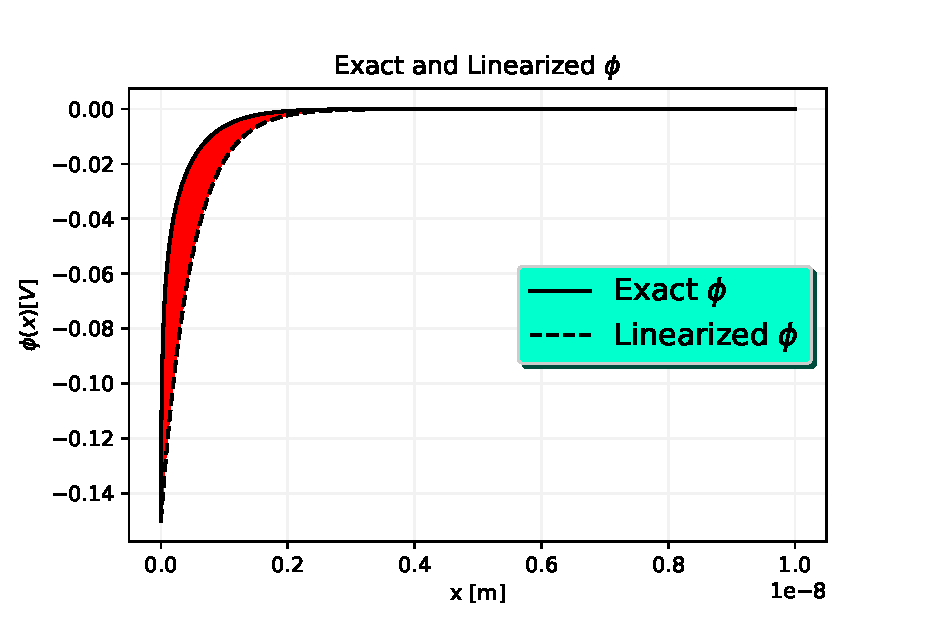
\includegraphics[width = 0.6\linewidth]{comparison-phi.eps}
 \caption{Comparison of the linearized PB solution with the analytical solution. The region in red is the error committed in this approximation}
\end{figure}

This results gives a good physical sense of how the potential should look like in a context of electrolyte solutions at equilibrium. We are interested in the dynamics of the system, though, so it makes sense to try to incorporate the current into Eq. \ref{eq:system}. In the next section we shall incorporate the current flowing through the interface as a border condition of Eq. \ref{eq:system}.

\section{Steady State Solution To The Diffusion-Reaction Problem}

In what follows, we shall assume that the system presents concentration gradients and
potential gradients along a single dimension $x$. This is equivalent to considering the interface infinitely large. Therefore, $\mathbf{N}_{+} = \hat{x}N_{+}$ and $\mathbf{N}_{-} = \hat{x}N_{-}$. 

In the steady state solution the concentration distribution of each electrolyte throughout the system should not change in time, thus

$$\frac{\partial C_+}{\partial t} = \frac{\partial C_-}{\partial t} = 0$$

This yields the following results

$$\nabla\cdot \mathbf{N}_+ = \frac{\partial N_{+}}{\partial x}=0$$
$$\nabla \cdot \mathbf{N}_- = \frac{\partial N_{-}}{\partial x}=0$$

Therefore, we have

$$N_+ = A_1$$
$$N_- = A_2$$

where $A_1$ and $A_2$ are constants determined by border conditions. Since the anion does not interact with the interface, we get after Eq.(\ref{eq_bc1})
$N_- = 0$. On the other hand, the flux due to the cation reaction with the interface ($Cu^{+2}\rightarrow Cu^{0}$) gives the boundary condition for $N_+$,

$$N_+ = \frac{I_0}{Az_+F}$$

The complete system of equations to be solved is

$$N_-(x) = 0$$

$$N_+(x) = \frac{I_0}{Aze}$$

\begin{figure}[h!]
\centering
	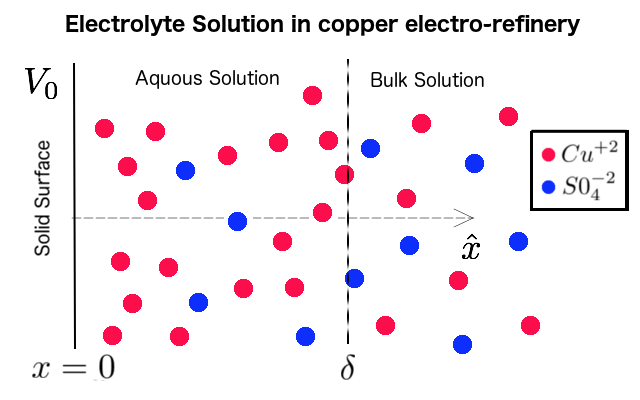
\includegraphics[width=0.5\textwidth]{geometry.png}
	\caption{Geometry of the problem. $x<\delta$ is the region of laminar. $x>\delta$ is the bulk of the solution. This image is for a value of $V_0<0$, such that the positive electrolytes distribute closer to the surface.}
\label{fig:geometry}
\end{figure}


According to Fig. \ref{fig:geometry}, for an interface area large compared to the laminar flux region we get the following equations 

\begin{eqnarray}\label{eq:system}
\frac{\partial C_+}{\partial x}-\frac{z F}{RT}C_+\frac{\partial \phi}{\partial x} &=& -\frac{I_0}{D_+Az_+ F}\label{eq:eq1} \\
\frac{\partial C_-}{\partial x}+\frac{z F}{RT}C_-\frac{\partial \phi}{\partial x} &=& 0 \label{eq:eq2}\\
\frac{\partial^2 \phi}{\partial x^2} &=& -\frac{1}{\epsilon} \sum_{s=\pm}z_s F C_s(x)\label{eq:eq3}
\end{eqnarray}

where A is the area of the interface electrode. 

To solve this system of partial differential equations, we will expand the concentration and the potential as a series in powers of $r = \frac{I_0}{D_+Az_+ F}$. We have

\begin{eqnarray}
C_s(x) = \sum_{n=0}^{\infty}r^n C_s^{(n)}(x)\\
\phi(x) = \sum_{n=0}^{\infty}r^n \phi^{(n)}(x)
\end{eqnarray}

Truncating the series at first order in $r$, we obtain the following system of equations to order zero in the current
\begin{eqnarray}
\frac{\partial C^{(0)}_+}{\partial x}-\frac{zF}{RT}C^{(0)}_+(x)\frac{\partial \phi^{(0)}}{\partial x} &=& 0\\
\label{eq:concentration-diff-zero1}
\frac{\partial C^{(0)}_-}{\partial x}+\frac{zF}{RT}C^{(0)}_-(x)\frac{\partial \phi^{(0)}}{\partial x}&=& 0\\
\label{eq:concentration-diff-zero2}
\frac{\partial^2  \phi^{(0)}}{\partial x^2} &=& -\frac{1}{\epsilon}\sum_{s= \pm} szF C^{(0)}_{s}(x)
\label{eq:concentration-diff-zero3}
\end{eqnarray}

and to first order in the current

\begin{eqnarray}
\frac{\partial C^{(1)}_+}{\partial x}-\frac{zF}{RT}\qty{C^{(1)}_+(x)\frac{\partial \phi^{(0)}}{\partial x}+C^{(0)}_+(x)\frac{\partial \phi^{(1)}}{\partial x}} &=& -1,\\
\label{eq:concentration-diff-first1}
\frac{\partial C^{(1)}_-}{\partial x}+\frac{zF}{RT}\qty{C^{(1)}_-(x)\frac{\partial \phi^{(0)}}{\partial x}+C^{(0)}_-(x)\frac{\partial \phi^{(1)}}{\partial x}}&=& 0,\\
\label{eq:concentration-diff-first2}
\frac{\partial^2  \phi^{(1)}}{\partial x^2} &=& -\frac{1}{\epsilon}\sum_{s= \pm} szF C^{(1)}_{s}(x).
\label{eq:concentration-diff-first3}
\end{eqnarray}




















\newpage

\section{Zero order solution to Poisson's equation for the electrolyte solution}
\label{sec:zeroorderphi}

We want to work with the dimensionless potential 

$$\Phi(x) = \frac{zF}{RT}\phi(x).$$

The zero order system can thus be written as

\begin{eqnarray}
\label{eq:zero-order}
C^{(0)}_+(x)'-C^{(0)}_+(x)\Phi^{(0)}(x)' &=& 0\\
 C^{(0)}_-(x)'+C^{(0)}_-(x)\Phi^{(0)}(x)'&=& 0\\
\Phi^{(0)}(x) ''&=& -\frac{(zF)^2}{RT\epsilon} (C^{(0)}_{+}(x)-C^{(0)}_{-}(x))
\end{eqnarray}



In this section we will solve equations \ref{eq:concentration-diff-first1} and \ref{eq:concentration-diff-first2}. 

From Eq. \ref{eq:zero-order},

$$\frac{\partial C^{(0)}_s}{\partial x}-sC^{(0)}_s\Phi^{(0)}(x)= 0$$

which yields

$$\int_{C_{b,s}}^{C^{(0)}_s(x)} \frac{dC^{(0)}_s}{C^{(0)}_s}=s\int_{\phi_b}^{\phi^{(0)}} d\Phi^{(0)}$$

where $\Phi_b = \Phi(\delta)$ is the potential at the bulk, which we will consider as the reference zero, $\phi_b = 0$. $C_{b,s}$ is the bulk concentration of each species in solution.

$$C^{(0)}_s(x)=C_{b,s}e^{s\Phi^{(0)}(x)}$$

Notice that 
\begin{equation}
C^{(0)}_s(\delta) = C_{b,s}e^{\frac{zF}{RT}\phi_b}=C_{b,s}.
\label{eq:zero-order-sol-c}
\end{equation}

Consider the bulk values of the concentration, $C_{s,b}$. In the bulk, the solution should be electrically neutral due to conservation of charge. Therefore, for a two electrolyte salt at the bulk

\begin{equation}
\label{eq:electroneutrality}
\sum_{s=\pm} C_{s,b} sz F = 0
\end{equation}


where $z$ is the valence of the electrolytes and $s = \pm$ is the sign of the charge of the electrolyte. $F = eN_A$ is the Faraday constant. From \ref{eq:electroneutrality} we get,

\begin{eqnarray}\nonumber
C_{b,+}Fz-C_{b,-}Fz=0\\
\rightarrow \frac{C_{b,+}}{C_{b,-}}=1
\label{eq:electroneutrality2}
\end{eqnarray}

$$C_{b,+}Fz-C_{b,-}Fz=0$$
$$\rightarrow \frac{C_{b,+}}{C_{b,-}}=1$$

In the case of a symmetric salt, $q_s=-q_{-s}$ (since in our notation $s=\pm$). Poisson's equation can be written (to zero order in the current) as

\begin{equation}
\label{eq:poisson1}
\frac{\partial^2 \Phi^{(0)}}{\partial x^2} = -\frac{zF}{\epsilon} \left(C_{b,+}e^{\Phi^{(0)}(x)}-C_{b,-}e^{-\Phi^{(0)}(x)}\right)
\end{equation}

where $z=|z_-|=|z_+|$. From equations \ref{eq:zero-order-sol-c}  and \ref{eq:electroneutrality2} we have $C_{b,+}=C_{b,+} = C_b$. Equation \ref{eq:poisson1} can be written in terms of the hyperbolic sine,

\begin{equation}
\label{eq:poisson2}
\frac{\partial^2 \Phi^{(0)}}{\partial x^2} = 2\frac{(zF)^2C_b}{RT\epsilon}\sinh{\left(\Phi^{(0)}(x)\right)}
\end{equation}

We define the quantity  

$$\kappa^2  = \frac{(zF)^2C_b}{RT\epsilon}$$

\begin{equation}
\frac{\partial^2 \Phi^{(0)}}{\partial x^2} = 2\kappa \sinh{\left(\Phi^{(0)}(x)\right)}
\end{equation}

We want to change variables to the dimensionless quantity $\kappa x$,

$$x \rightarrow \xi = \kappa x$$
 $$d \xi  = \kappa d x $$
 
Thus, we write,

\begin{equation}
\Phi^{(0)}(\xi)''= 2\sinh{\left(\Phi^{(0)}(\xi)\right)}
\end{equation}

Multiplying by  $\Phi'^{(0)}$ and integrating the equation over the interval $[\xi, \delta]$ we get,
 
\begin{align}
\Phi^{(0)}(\kappa \delta)'^2  -\Phi^{(0)}(\xi)'^2   = 2(cosh(\phi(\kappa \delta))-cosh(\phi(\xi)))
\end{align}

The border condition for the potential yields, 

$$\Phi^{(0)}(\xi)' \rightarrow 0.$$

Therefore

\begin{align}
\Phi^{(0)}(\xi)'^2   &= 2(\cosh(\phi(\xi))-1),\\
&= 4sinh^2(\phi(\xi)), \\
\rightarrow \Phi^{(0)} &= \pm 2\sinh(\phi(\xi).
\label{eq:phiprime}
\end{align}


The border conditions for the potential are $\Phi^{(0)}(0) = \bar{V}_0<0$ and $\Phi^{(0)}(\kappa \delta) = 0$, the slope of $\Phi^{(0)}$ must be positive and decreasing. This yields the positive solution to equation \ref{eq:phiprime}
\begin{align}
\Phi^{(0)} &=  2\sqrt{\sinh(\phi(\xi))}.
\end{align}

This is a separable equation which can be integrated directly, yielding

\begin{align}
	\log\qty{\frac{1-e^{\Phi^{(0)}/2}}{1+e^{\Phi^{(0)}/2}}} = -\xi + C,
\end{align}

\begin{align}
	\rightarrow \frac{1-e^{\Phi^{(0)}/2}}{1+e^{\Phi^{(0)}/2}}= Ae^{-\xi}.
\end{align}

It can be found using the border condition $\Phi^{(0)}(0) = \bar{V}_0$

\begin{align}
A = \tanh\qty{{\bar{V}_0/4}}
\end{align}

Solving for $\Phi^{(0)}$,

\begin{align}
\Phi^{(0)}(\xi) =  2\log{\qty{\tanh\qty{\frac{\xi-\xi_0}{2}}}},
\label{eq:pot0}
\end{align}

where we have defined

$$.$$

The minus sign in the previous definition is due to the fact that $\bar{V}_0 < 0$ for our case.




\section{Charge Density At The Interface}

From equation \ref{eq:pot0} we can obtain the electric field, which in terms of $x$ has the form

\begin{align}
E(x) =  \frac{2\kappa}{\beta q} \csc\qty{\kappa(x-x_0)},
\label{eq:pot0}
\end{align}

where

\begin{align}
e^{\xi_0} = -\tanh\qty{\frac{\bar{V}_0}{4}}.
\label{eq:expz0}
\end{align}

From electrostatics we know that the border condition for the electric field at a conductors interface is
\begin{align}
	E(x)\big|_{interface} = \frac{\sigma}{\epsilon}.
\end{align}

We thus obtain the surface charge in terms of the voltage at the interface

\begin{align}
	\sigma = -\frac{2 \epsilon \kappa}{\beta q} \csc\qty{kz_0},
\end{align}

which using Eq. \ref{eq:expz0} can be written as

\begin{align}
	\sigma(V_0) = -\frac{2 \epsilon \kappa}{\beta q} \frac{\tanh\qty{\frac{q\beta V_0}{4}}}{\tanh\qty{\frac{q\beta V_0}{4}}-1}
\end{align}

This equation can be solved for $V_0$ in terms of the surface charge density $\sigma$

\begin{align}
	V_0 = \tanh^{-1}\qty{-\frac{8\epsilon\kappa}{(q \beta)^2 \sigma} \qty{1 \pm \frac{1}{2}\sqrt{1+\frac{\beta^2 q^2\sigma^2}{\epsilon^2\kappa^2}}}}
\end{align}


\begin{figure}[htbp!]
\centering
\begin{subfigure}{.4\textwidth}
  \centering
  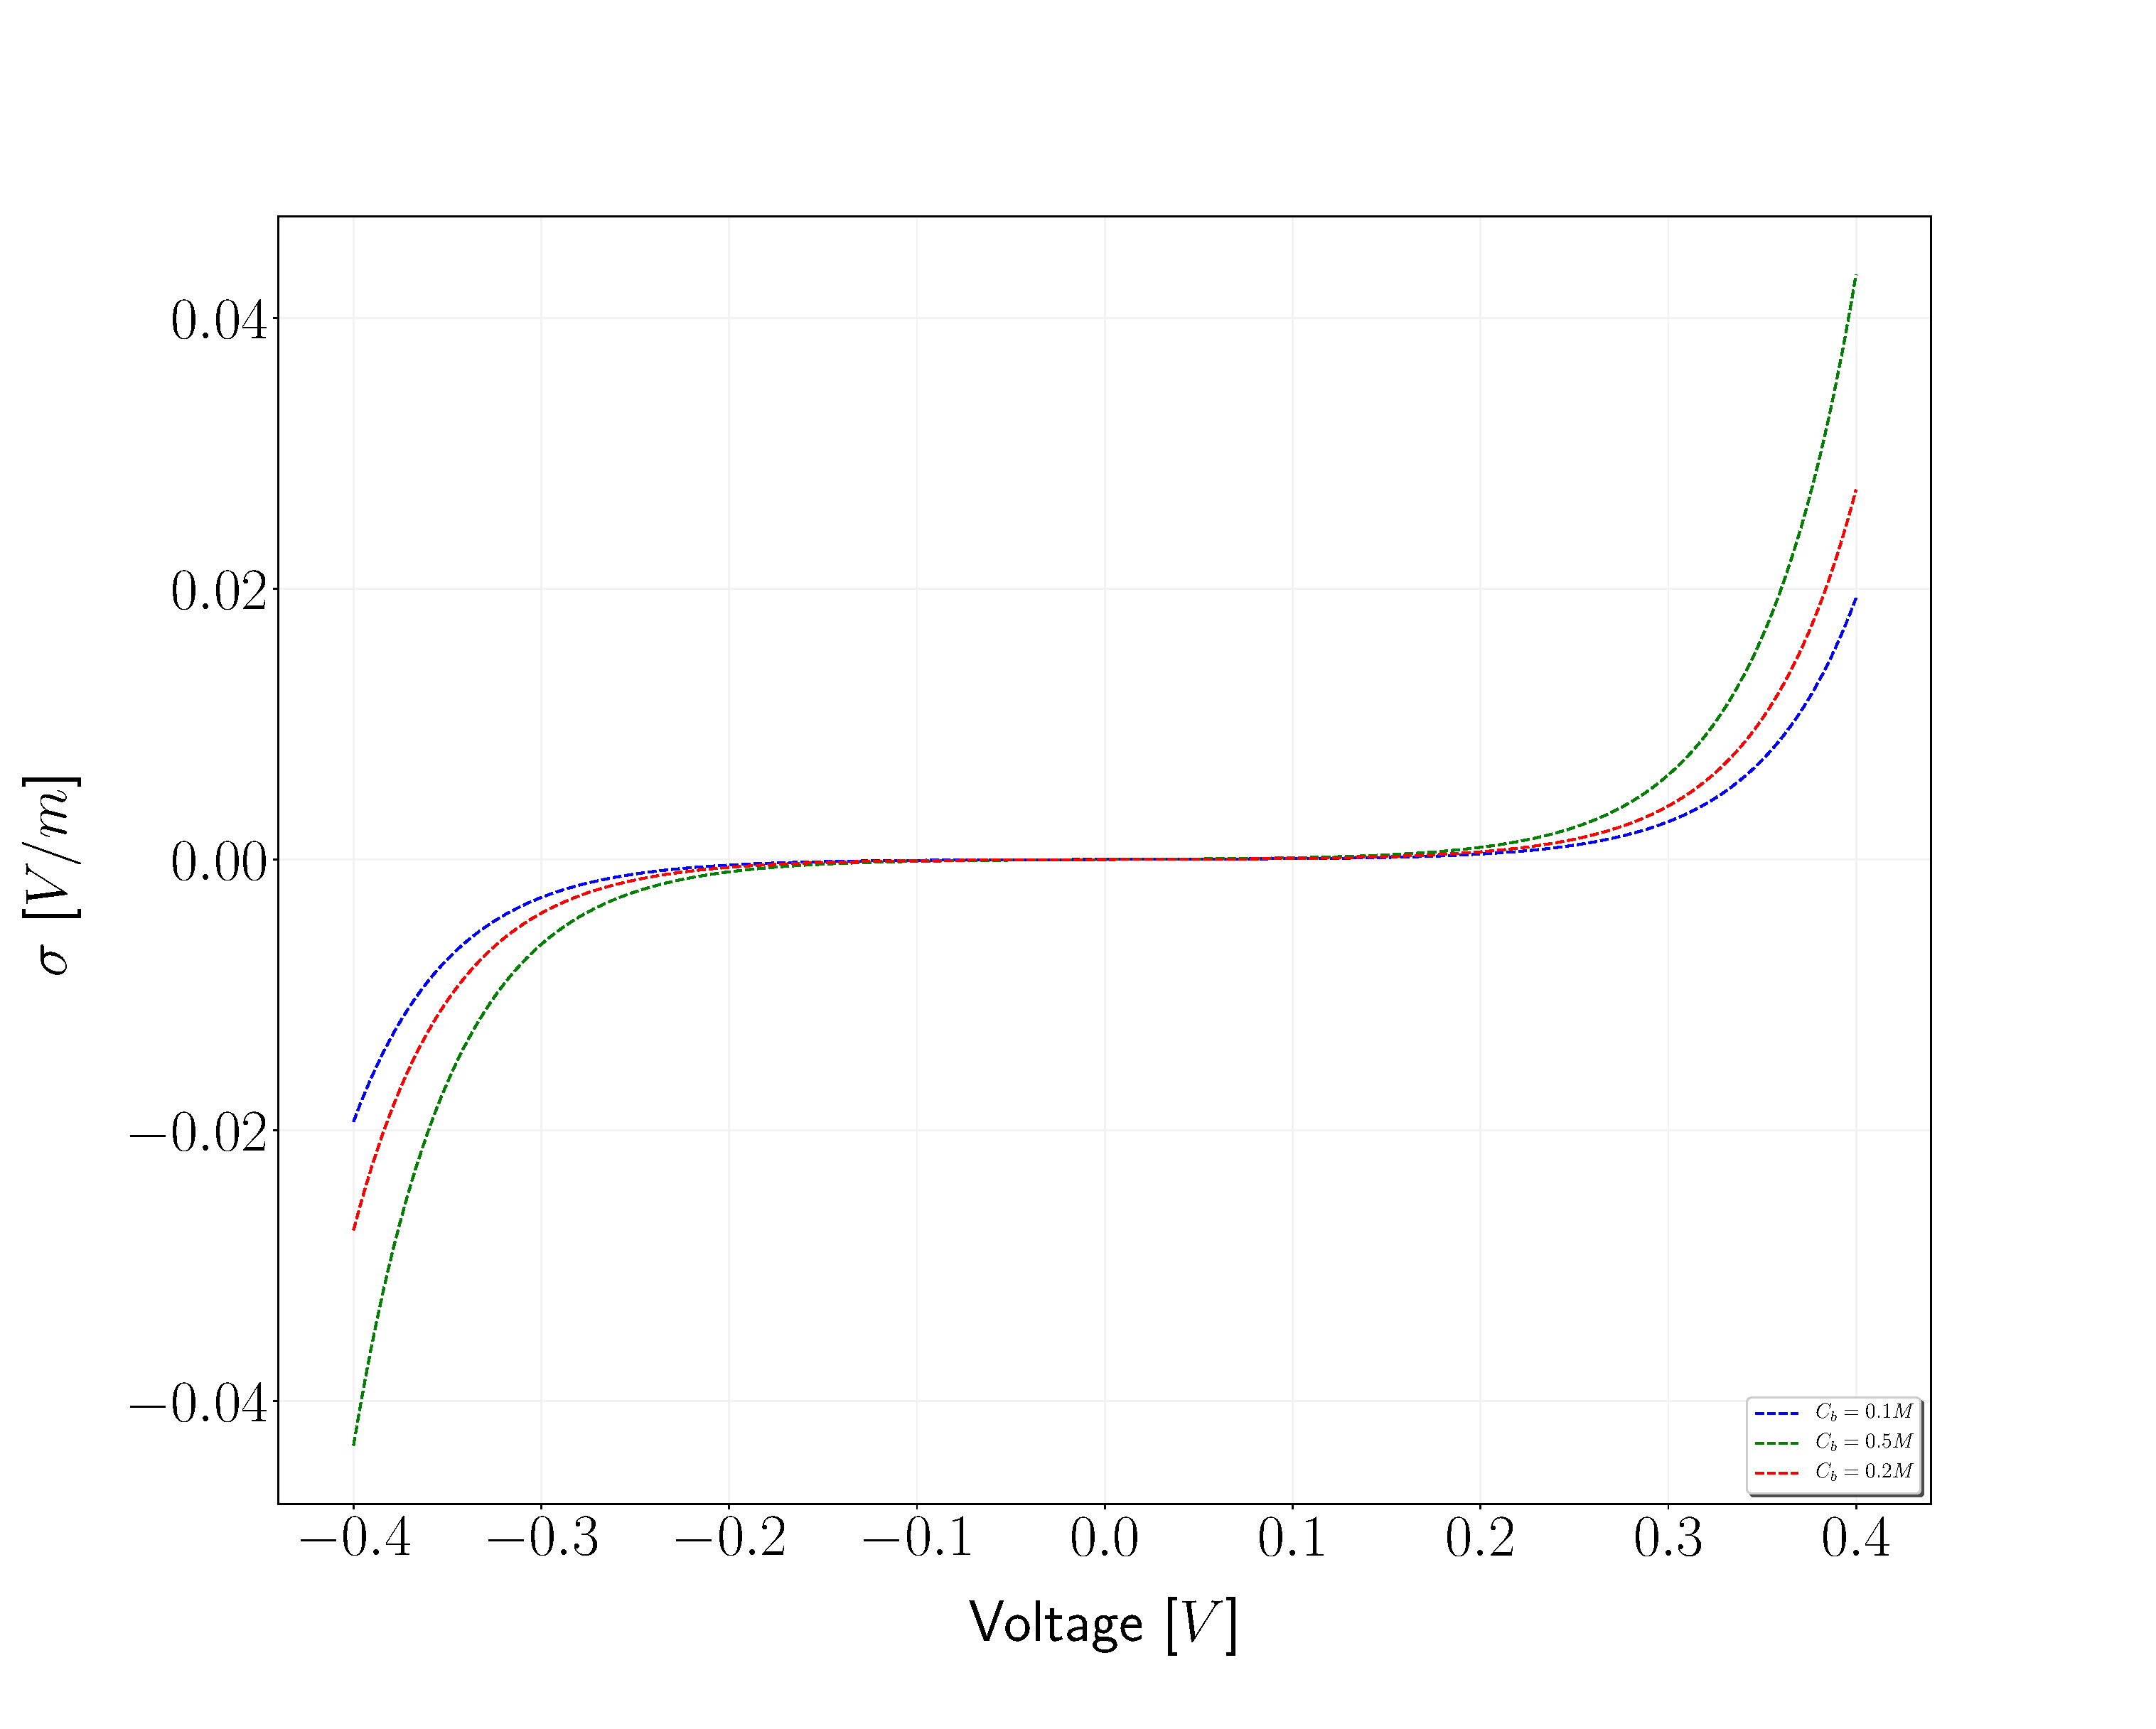
\includegraphics[width=\linewidth]{sigma-voltage.eps}
  \caption{}
  \label{fig:sub1}
\end{subfigure}%
\begin{subfigure}{.4\textwidth}
  \centering
  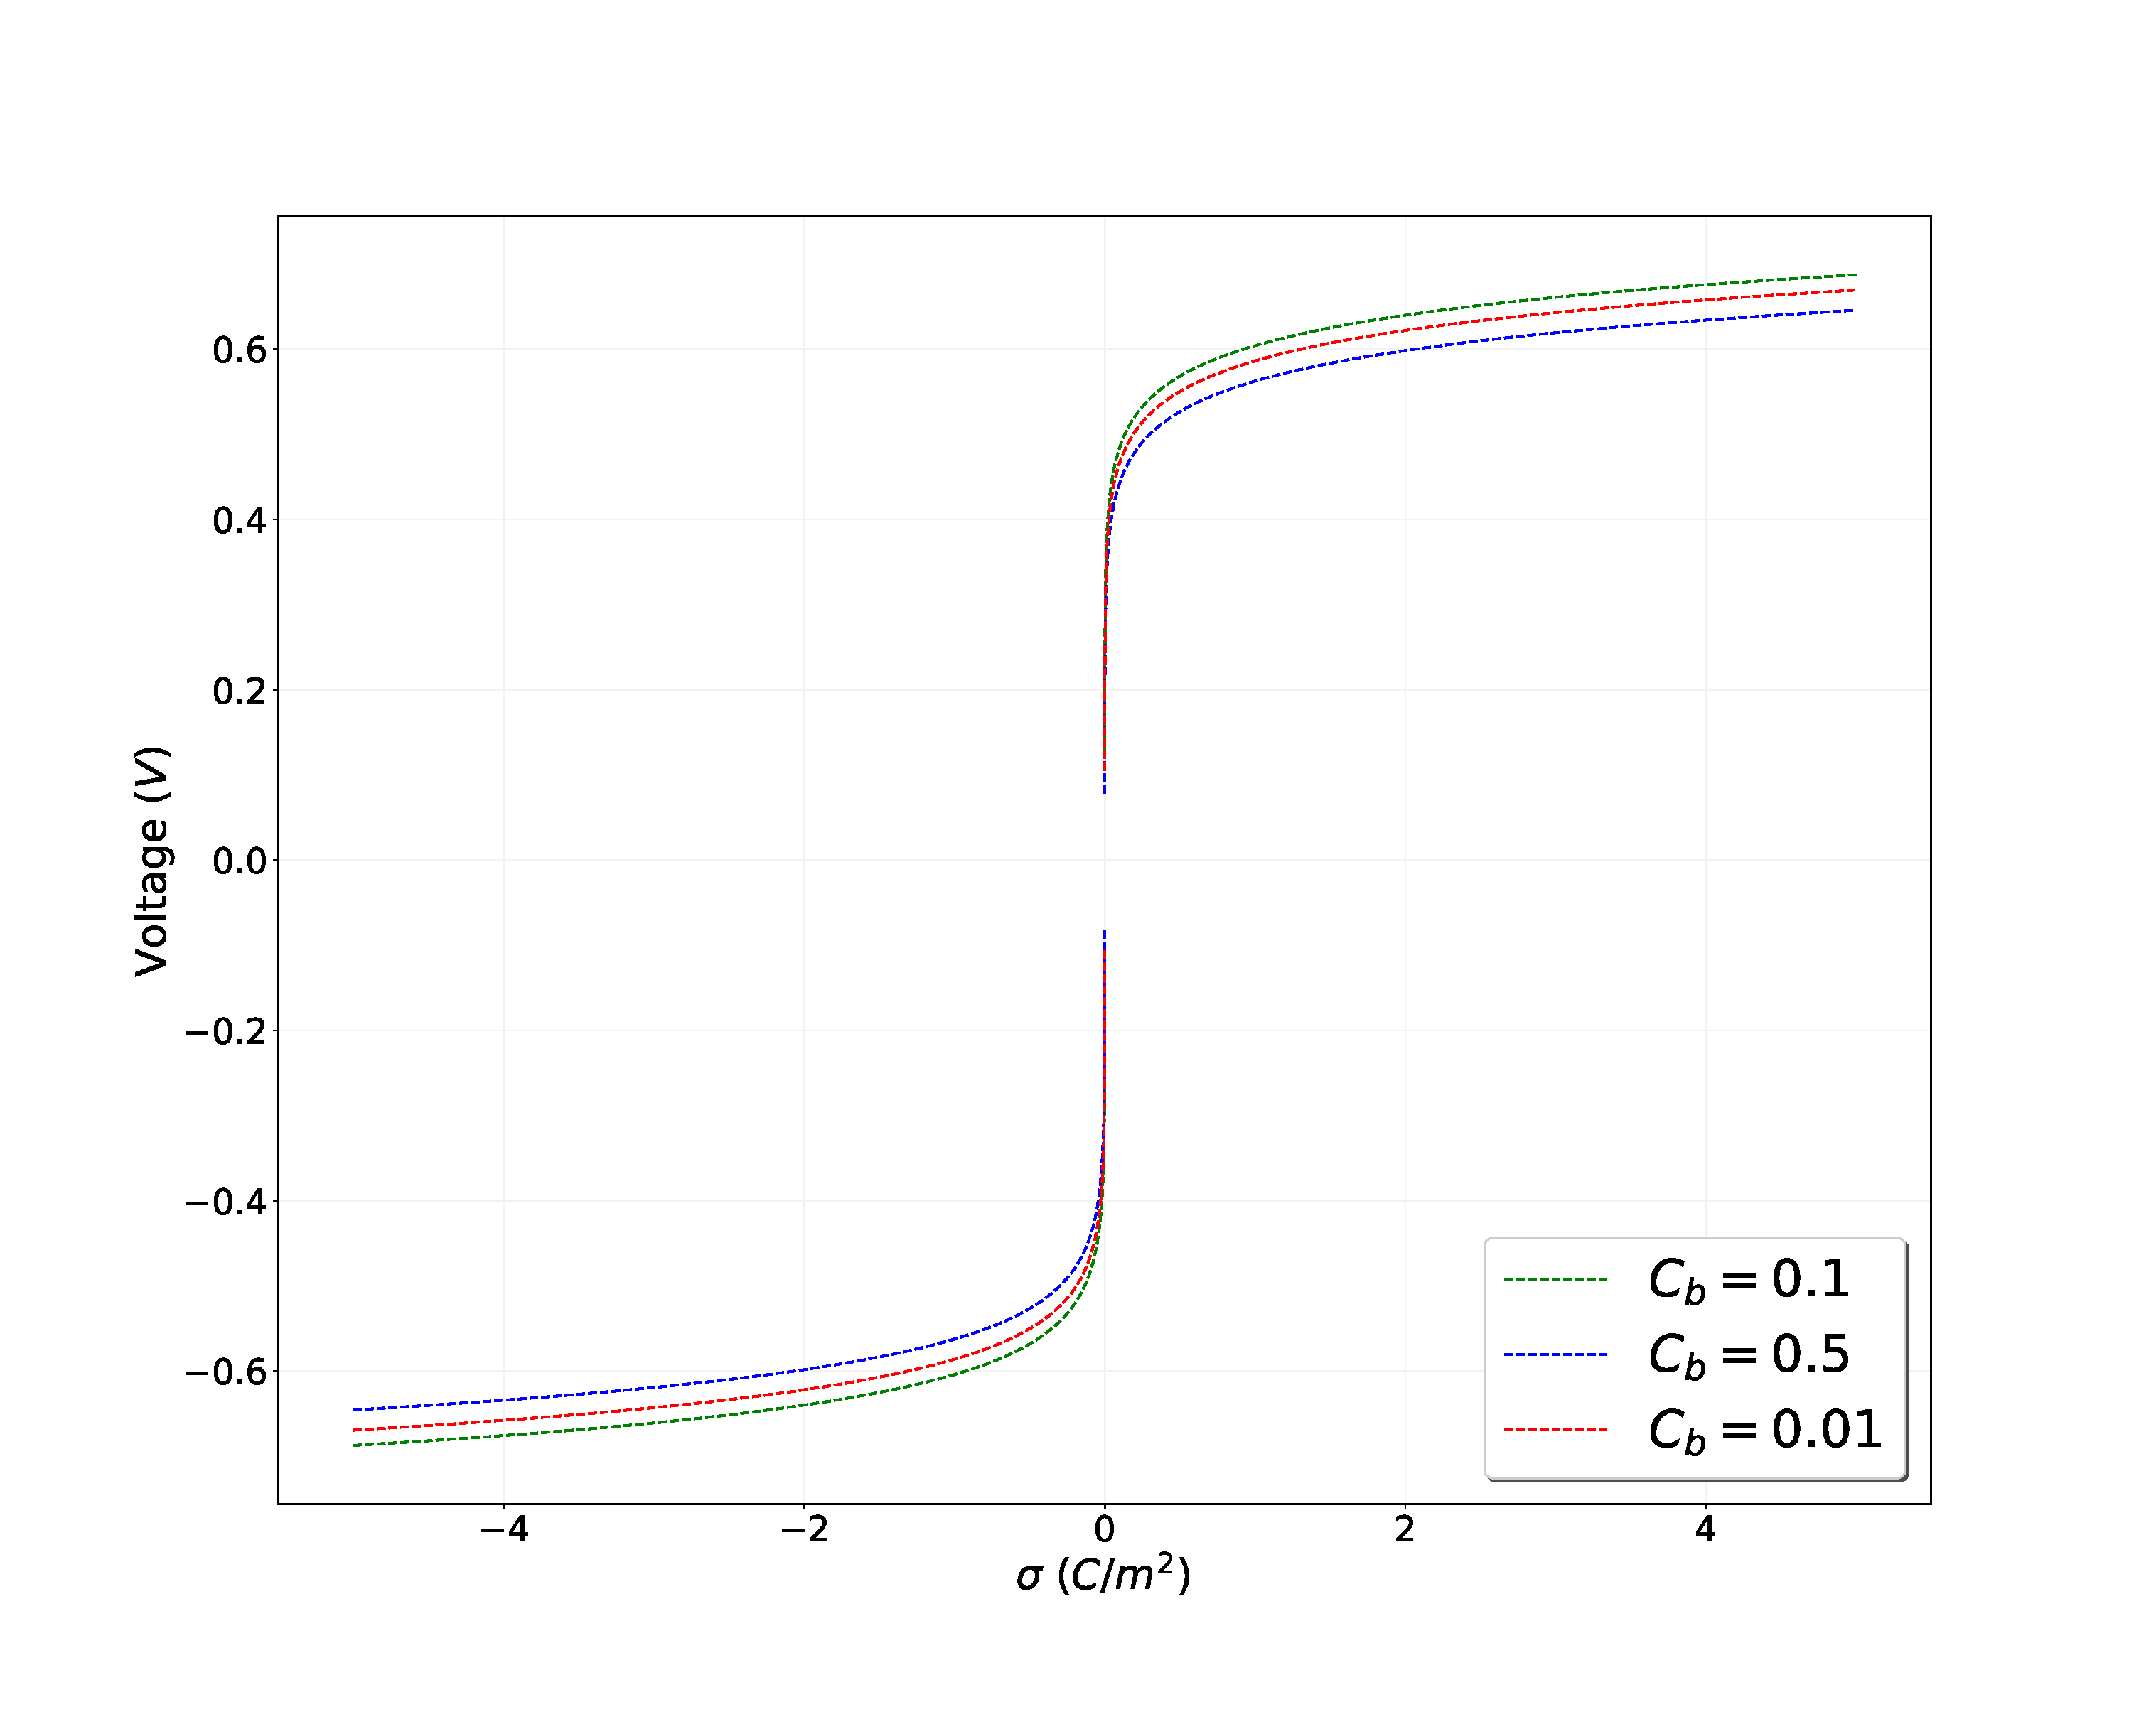
\includegraphics[width=\linewidth]{voltage-sigma.eps}
  \caption{}
  \label{fig:sub2}
\end{subfigure}
\caption{\textbf{(a)} Surface charge density in terms of the potential border condition. \textbf{(b)} Inverse of (a)}
\label{fig:test}
\end{figure}

\begin{figure}[htbp!]
\centering
\begin{subfigure}{.4\textwidth}
  \centering
  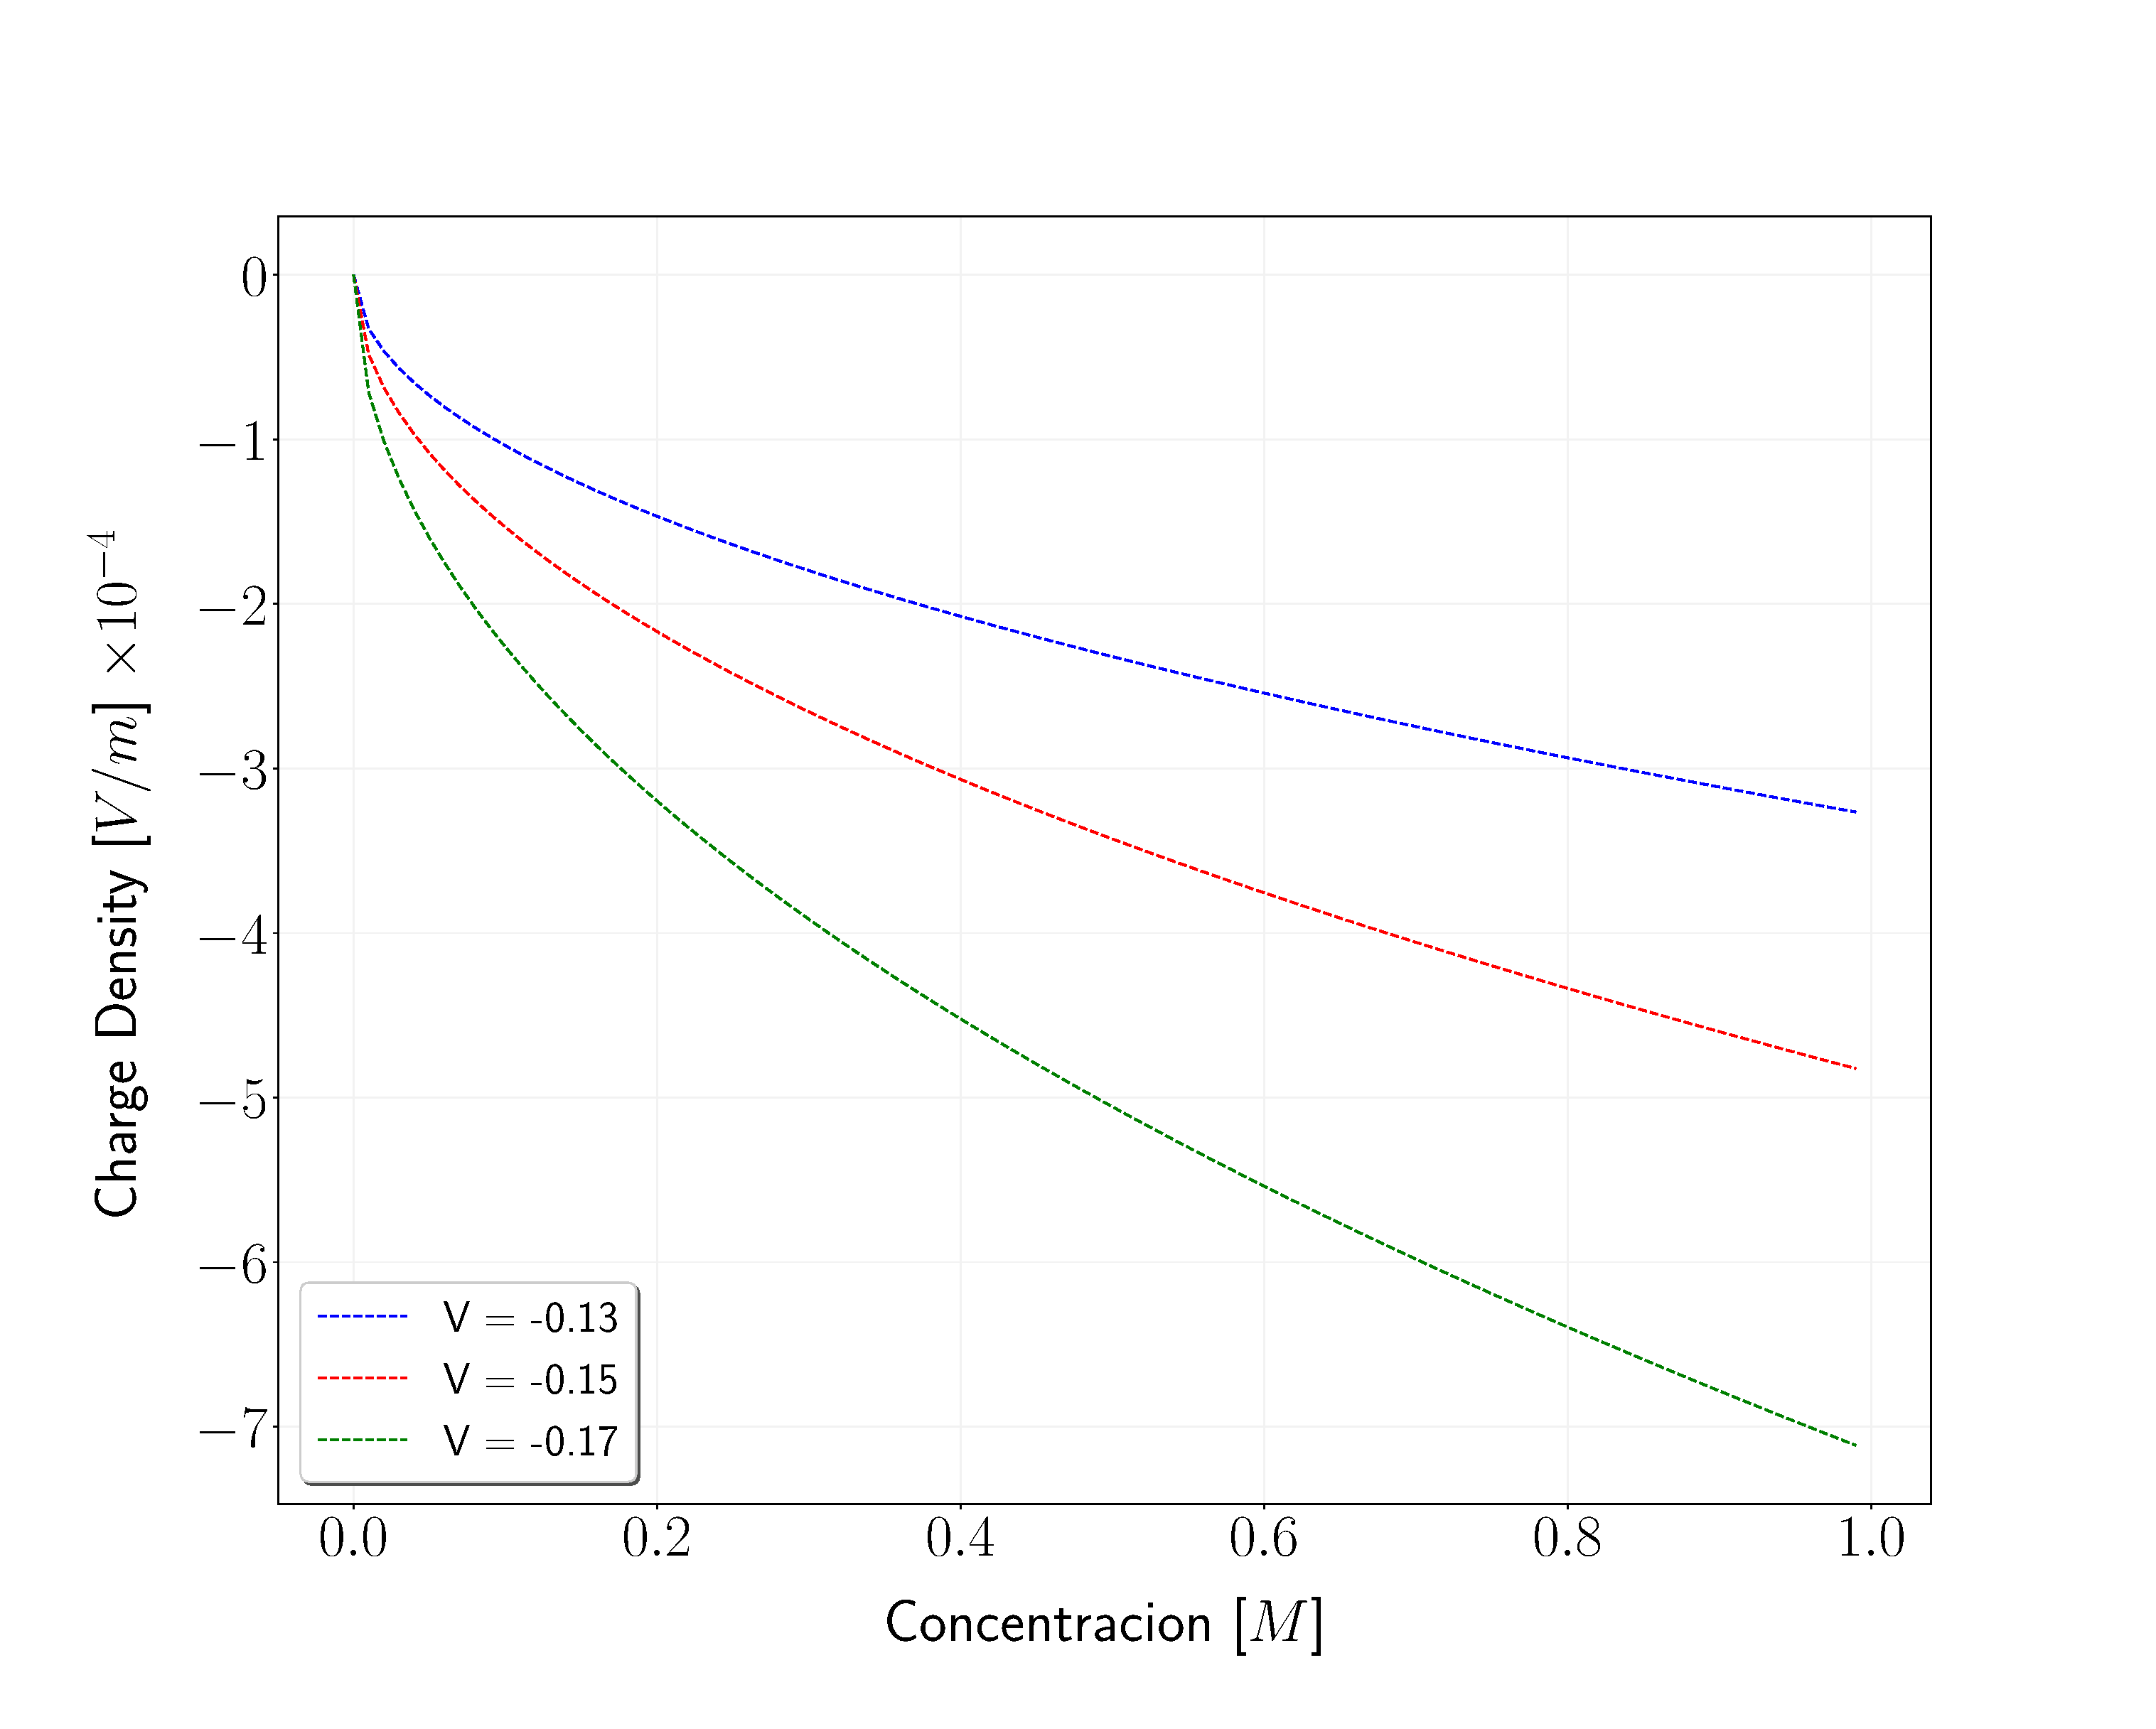
\includegraphics[width=\linewidth]{sigma-concentration.eps}
  \caption{}
  \label{fig:sub1}
\end{subfigure}%
\begin{subfigure}{.4\textwidth}
  \centering
  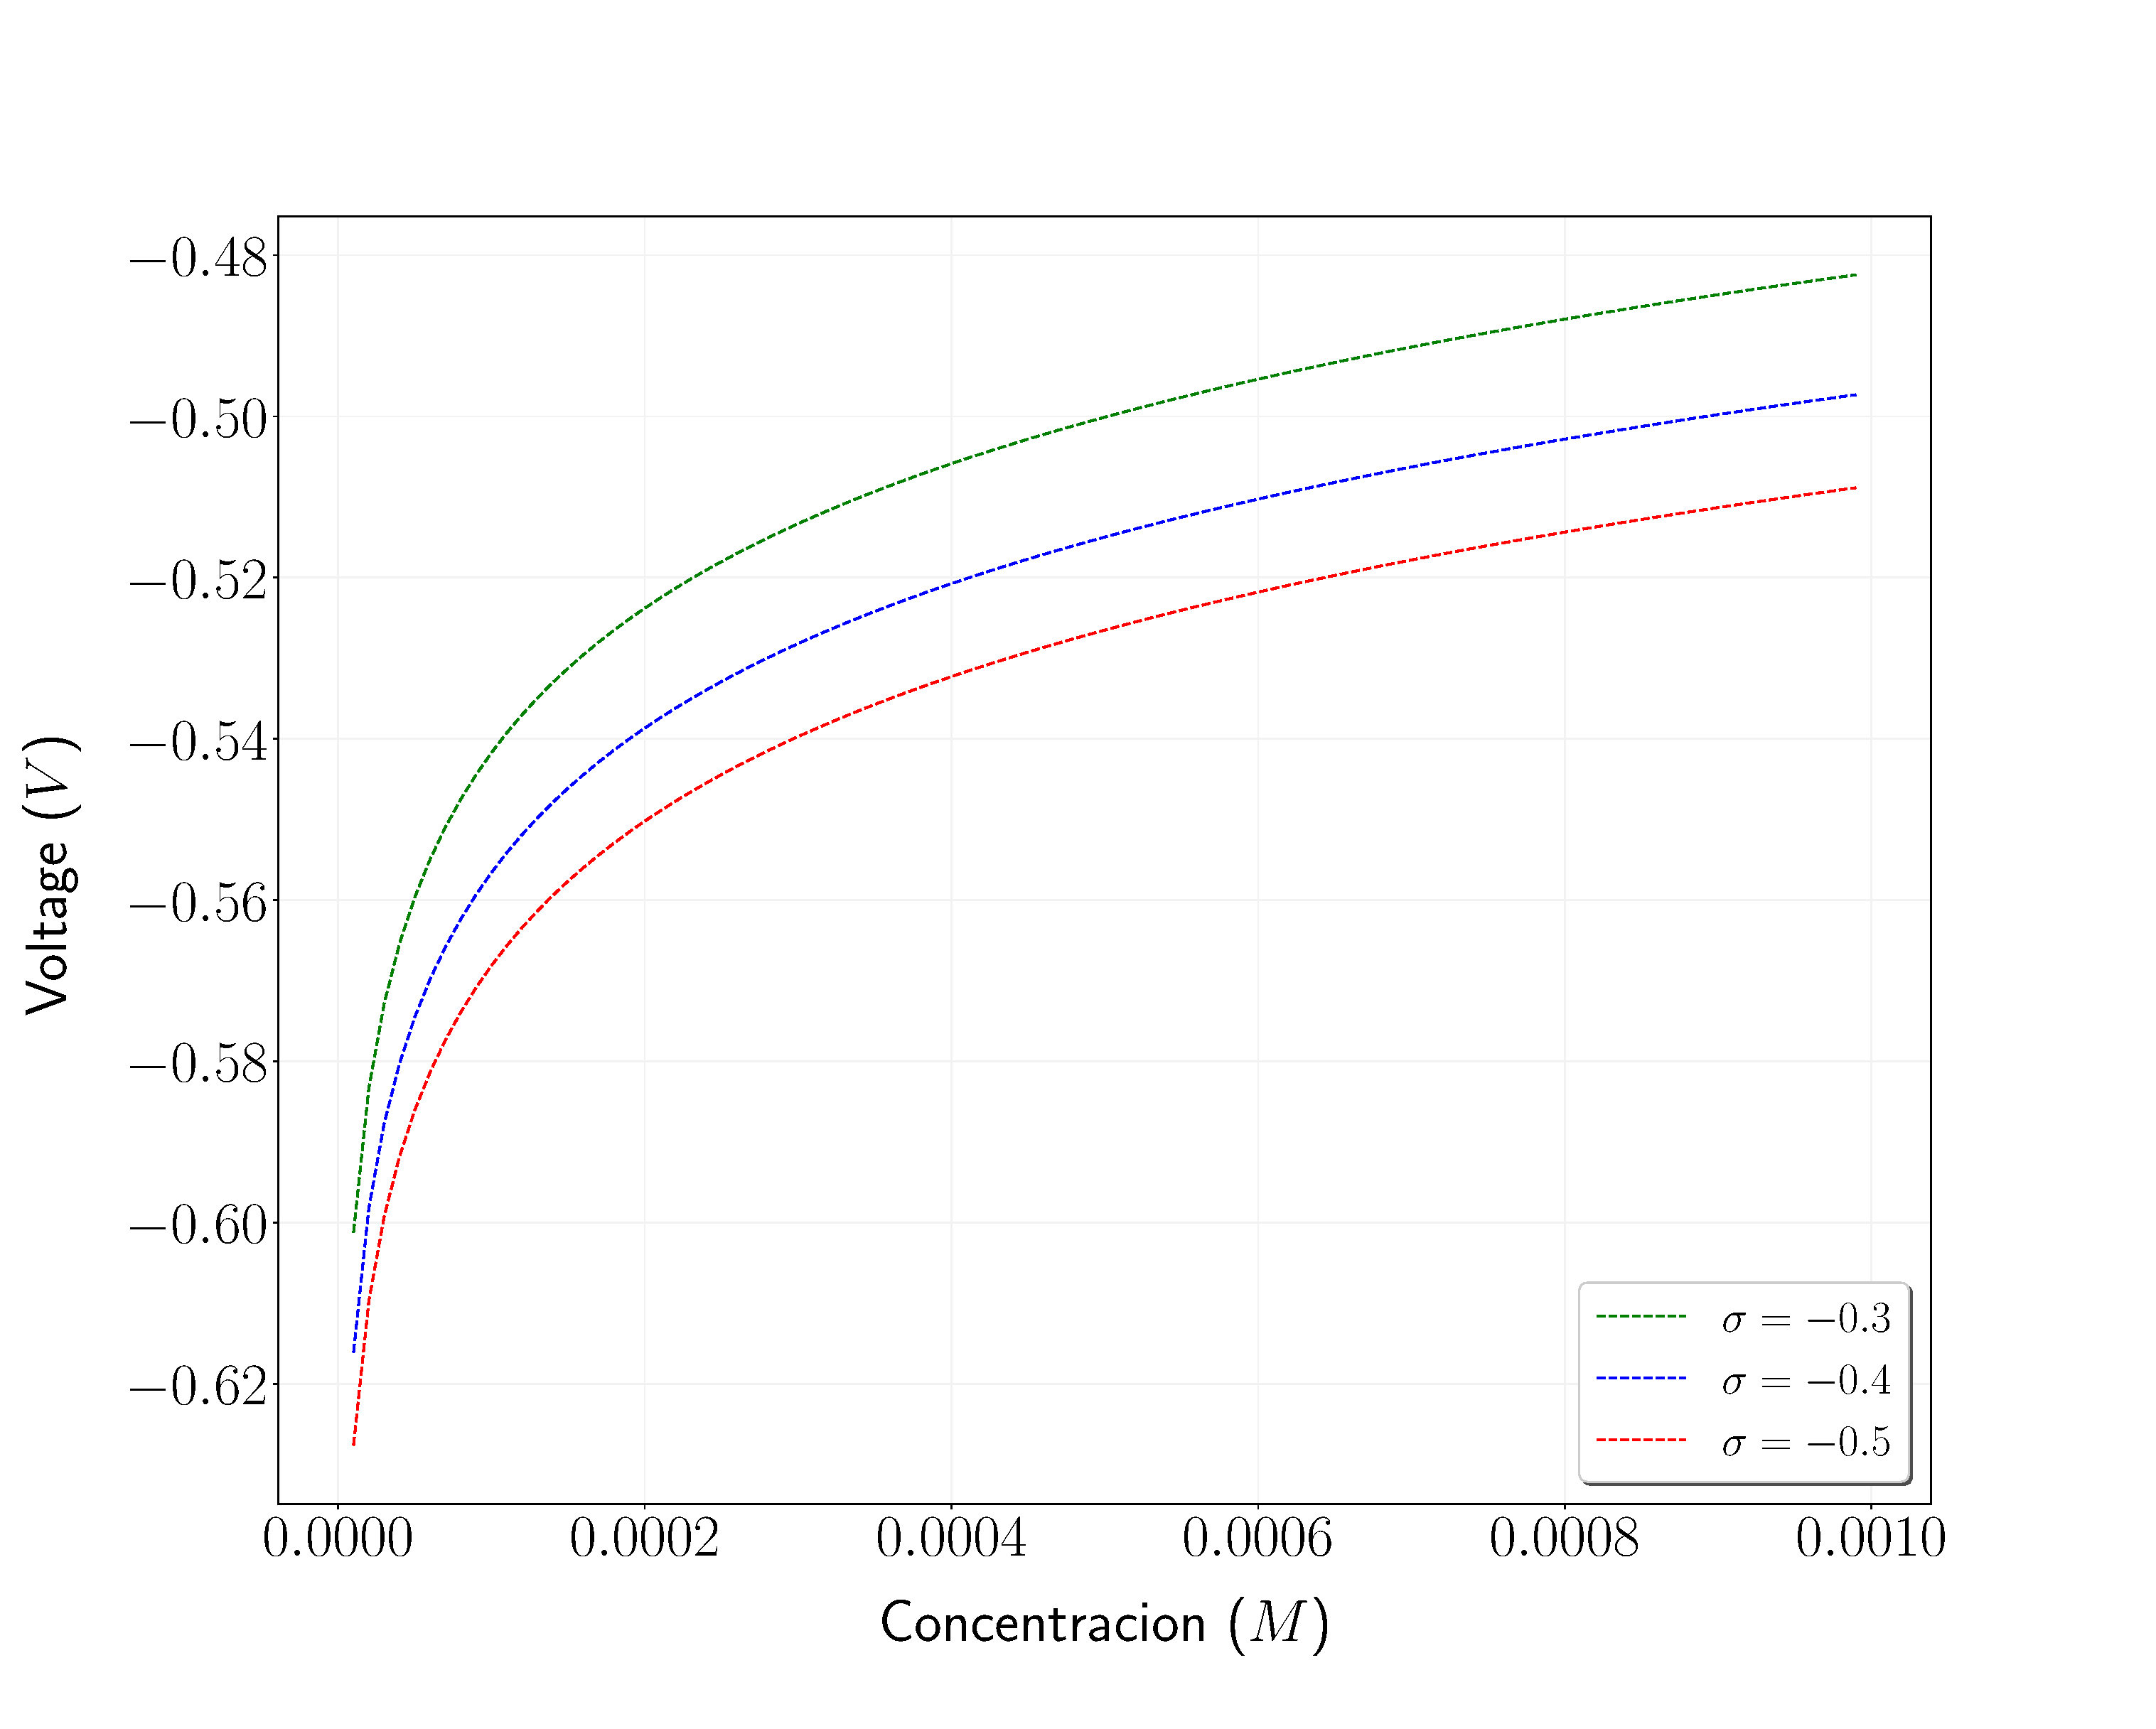
\includegraphics[width=\linewidth]{voltage-concentration.eps}
  \caption{}
  \label{fig:sub2}
\end{subfigure}
\caption{\textbf{(a)} Surface charge density in terms of the bulk concentration. \textbf{(b)} Voltage at the interface in terms of the bulk concentration (a)}
\label{fig:test}
\end{figure}




\section{Solution to the concentration at first order in the current $I_0$}


Now we solve Equation \ref{eq:system} at first order in the current $I_0$. From Eq. \ref{eq:concentration-diff-first2}, we consider the term proportional to $\frac{\partial \phi^{(1)}}{\partial x}$ such that

\begin{equation}
\bigg|\frac{\partial \phi^{(1)}}{\partial x}\bigg| << \frac{\kappa V_0}{r},
\label{eq:approx}
\end{equation}

since the gradient of the correction to the potential should be negligible compared to the gradient of the zero order contribution. This will be shown later in a numerical analysis. With this approximation, the system to first order in $r$ becomes

\begin{eqnarray}
\frac{\partial C^{(1)}_+}{\partial \xi}-C^{(1)}_+(\xi)\frac{\partial \Phi^{(0)}}{\partial \xi} &=& -\frac{1}{\kappa} \\
\label{eq:concentration-diff-first4}
\frac{\partial C^{(1)}_-}{\partial \xi}+C^{(1)}_-(\xi)\frac{\partial \Phi^{(0)}}{\partial \xi} &=& 0 \\
\label{eq:concentration-diff-first5}
\frac{\partial^2  \phi^{(1)}}{\partial \xi^2} &=& -(C^{(1)}_{+}(\xi)-C^{(1)}_{-}(\xi))
\label{eq:concentration-diff-first6}
\end{eqnarray}


In Eq. \ref{eq:concentration-diff-first4}, we obtain

$$\frac{\partial C^{(1)}_+}{\partial \xi}-C^{(1)}_+\frac{\partial \Phi^{(0)}}{\partial \xi} = -\frac{1}{\kappa}$$

Using an integrating factor of the form
$$\mu(\xi)=e^{-\int_{\kappa\delta}^\xi \frac{zF}{RT}\frac{d\phi^{(0)}}{d\xi'}d\xi'}=e^{- (\Phi^{(0)}(\xi)-\phi_b)} = e^{-\Phi^{(0)}(\xi)}$$

We can write \ref{eq:concentration-diff-first4}  as

$$\frac{d}{d\xi}\left(C^{(1)}_+(\xi)\mu(\xi) \right)=-\frac{\mu(\xi)}{\kappa},$$

where $z=|z_\pm|$. Integrating over $x$ and considering that $C^{(1)}_+(\xi)\mu(\xi)\big|_{\xi \rightarrow \infty} = C^{(1)}_{+,b} = 0$ due to border conditions, we get

$$C^{(1)}_+(\xi) =\frac{1}{\kappa\mu(\xi)}\int_{0}^{\xi}\mu(\xi')d\xi'$$

Eq. \ref{eq:concentration-diff-first5} can be integrated by separation of variables, and the solution is 

$$C^{(1)}_-(\xi) = C^{(1)}_{b,-}e^{\phi^{(0)}(\xi)}.$$

Since our border condition yields $ C^{(1)}_{b,-} = 0$, the contribution to first order of the negative ion concentration is zero. 

Computing the integral, we find to first order in the current the following solutions for the concentrations.

\begin{eqnarray}
C^{(1)}_+(\xi) &=& -\frac{1}{\kappa} \qty{\xi_\delta-\xi-\frac{2}{\gamma}}\tanh^2\qty{\frac{\xi-\xi_0}{2}}+2\tanh\qty{\frac{\xi-\xi_0}{2}}\\
C^{(1)}_-(\xi) &=& 0
\label{eq:firstordersol}
\end{eqnarray}



\section{Potential to first order in the current}

Now we need to solve Eq. \ref{eq:concentration-diff-first6}
\begin{eqnarray}
\frac{\partial^2  \Phi^{(1)}}{\partial \xi^2} &=& -(C^{(1)}_{+}(\xi)-C^{(1)}_{-}(\xi)).
\end{eqnarray}

Expanding, we have 

\begin{eqnarray}\nonumber
\frac{\partial^2  \Phi^{(1)}}{\partial \xi^2} &=& -C^{(1)}_{+}(\xi)\\
&=& -\frac{1}{\kappa} \qty{\xi_\delta-\xi-\frac{2}{\gamma}}\tanh^2\qty{\frac{\xi-\xi_0}{2}}+2\tanh\qty{\frac{\xi-\xi_0}{2}}
\end{eqnarray}


Integrating twice and using the fact that $\Psi'^{(1)} = 0$, $\Psi^{(1)} = 0$ we obtain

\begin{eqnarray}
\Phi'^{(1)}(\xi) = \frac{1}{\kappa} \qty{A + B\xi + C\xi^2 + D \tanh{\frac{\xi-\xi_0}{2}}+E\xi\tanh{\frac{\xi-\xi_0}{2}}} 
\end{eqnarray}


And 

\begin{eqnarray}
\Phi^{(1)}(\xi) = -\frac{1}{\kappa} (A(\xi_\delta - \xi) + \frac{B}{2}(\xi_\delta^2-\xi^2) + \frac{C}{3}(\xi_\delta^3 - \xi^3) + \\
D\log\bigg|\frac{\cosh{\frac{\xi_\delta-\xi}{2}}}{\cosh{\frac{\xi-\xi}{2}}}\bigg| + E \qty{\xi_\delta\log|\cosh\qty{\frac{\xi_\delta-\xi_0}{2}}-\xi\log|\cosh\qty{\frac{\xi-\xi_0}{2}}}-EI_\delta(\xi)
\end{eqnarray}


where

\begin{eqnarray*}
	A = 2\gamma\xi_\delta - \frac{2\xi_\delta}{\gamma} - 2 \gamma - \frac{\xi_\delta^2}{2},\\
	B = -\qty{\xi_\delta -\frac{2}{\gamma}},\\
	C = \frac{3}{2}\\
	D = -2 \qty{\xi_\delta - \frac{2}{\gamma}},\\
	E = 2,\\
	\gamma = \tanh\qty{\frac{\xi_0}{2}},
\end{eqnarray*}

and

\begin{align}
	I_\delta(\xi) = \int_\xi^{\xi_\delta} \log\bigg|\cosh\qty{\frac{\xi-\xi_0}{2}}\bigg| d\xi.
\end{align}




This integral must be evaluated numerically for each value of $\xi$. In order to do this, we use the Simpson Rule. Fig. \ref{fig:analytic-results} shows the potential to first order in the current alongside with the zero order potential. 


\begin{figure}[h!]
 \centering
 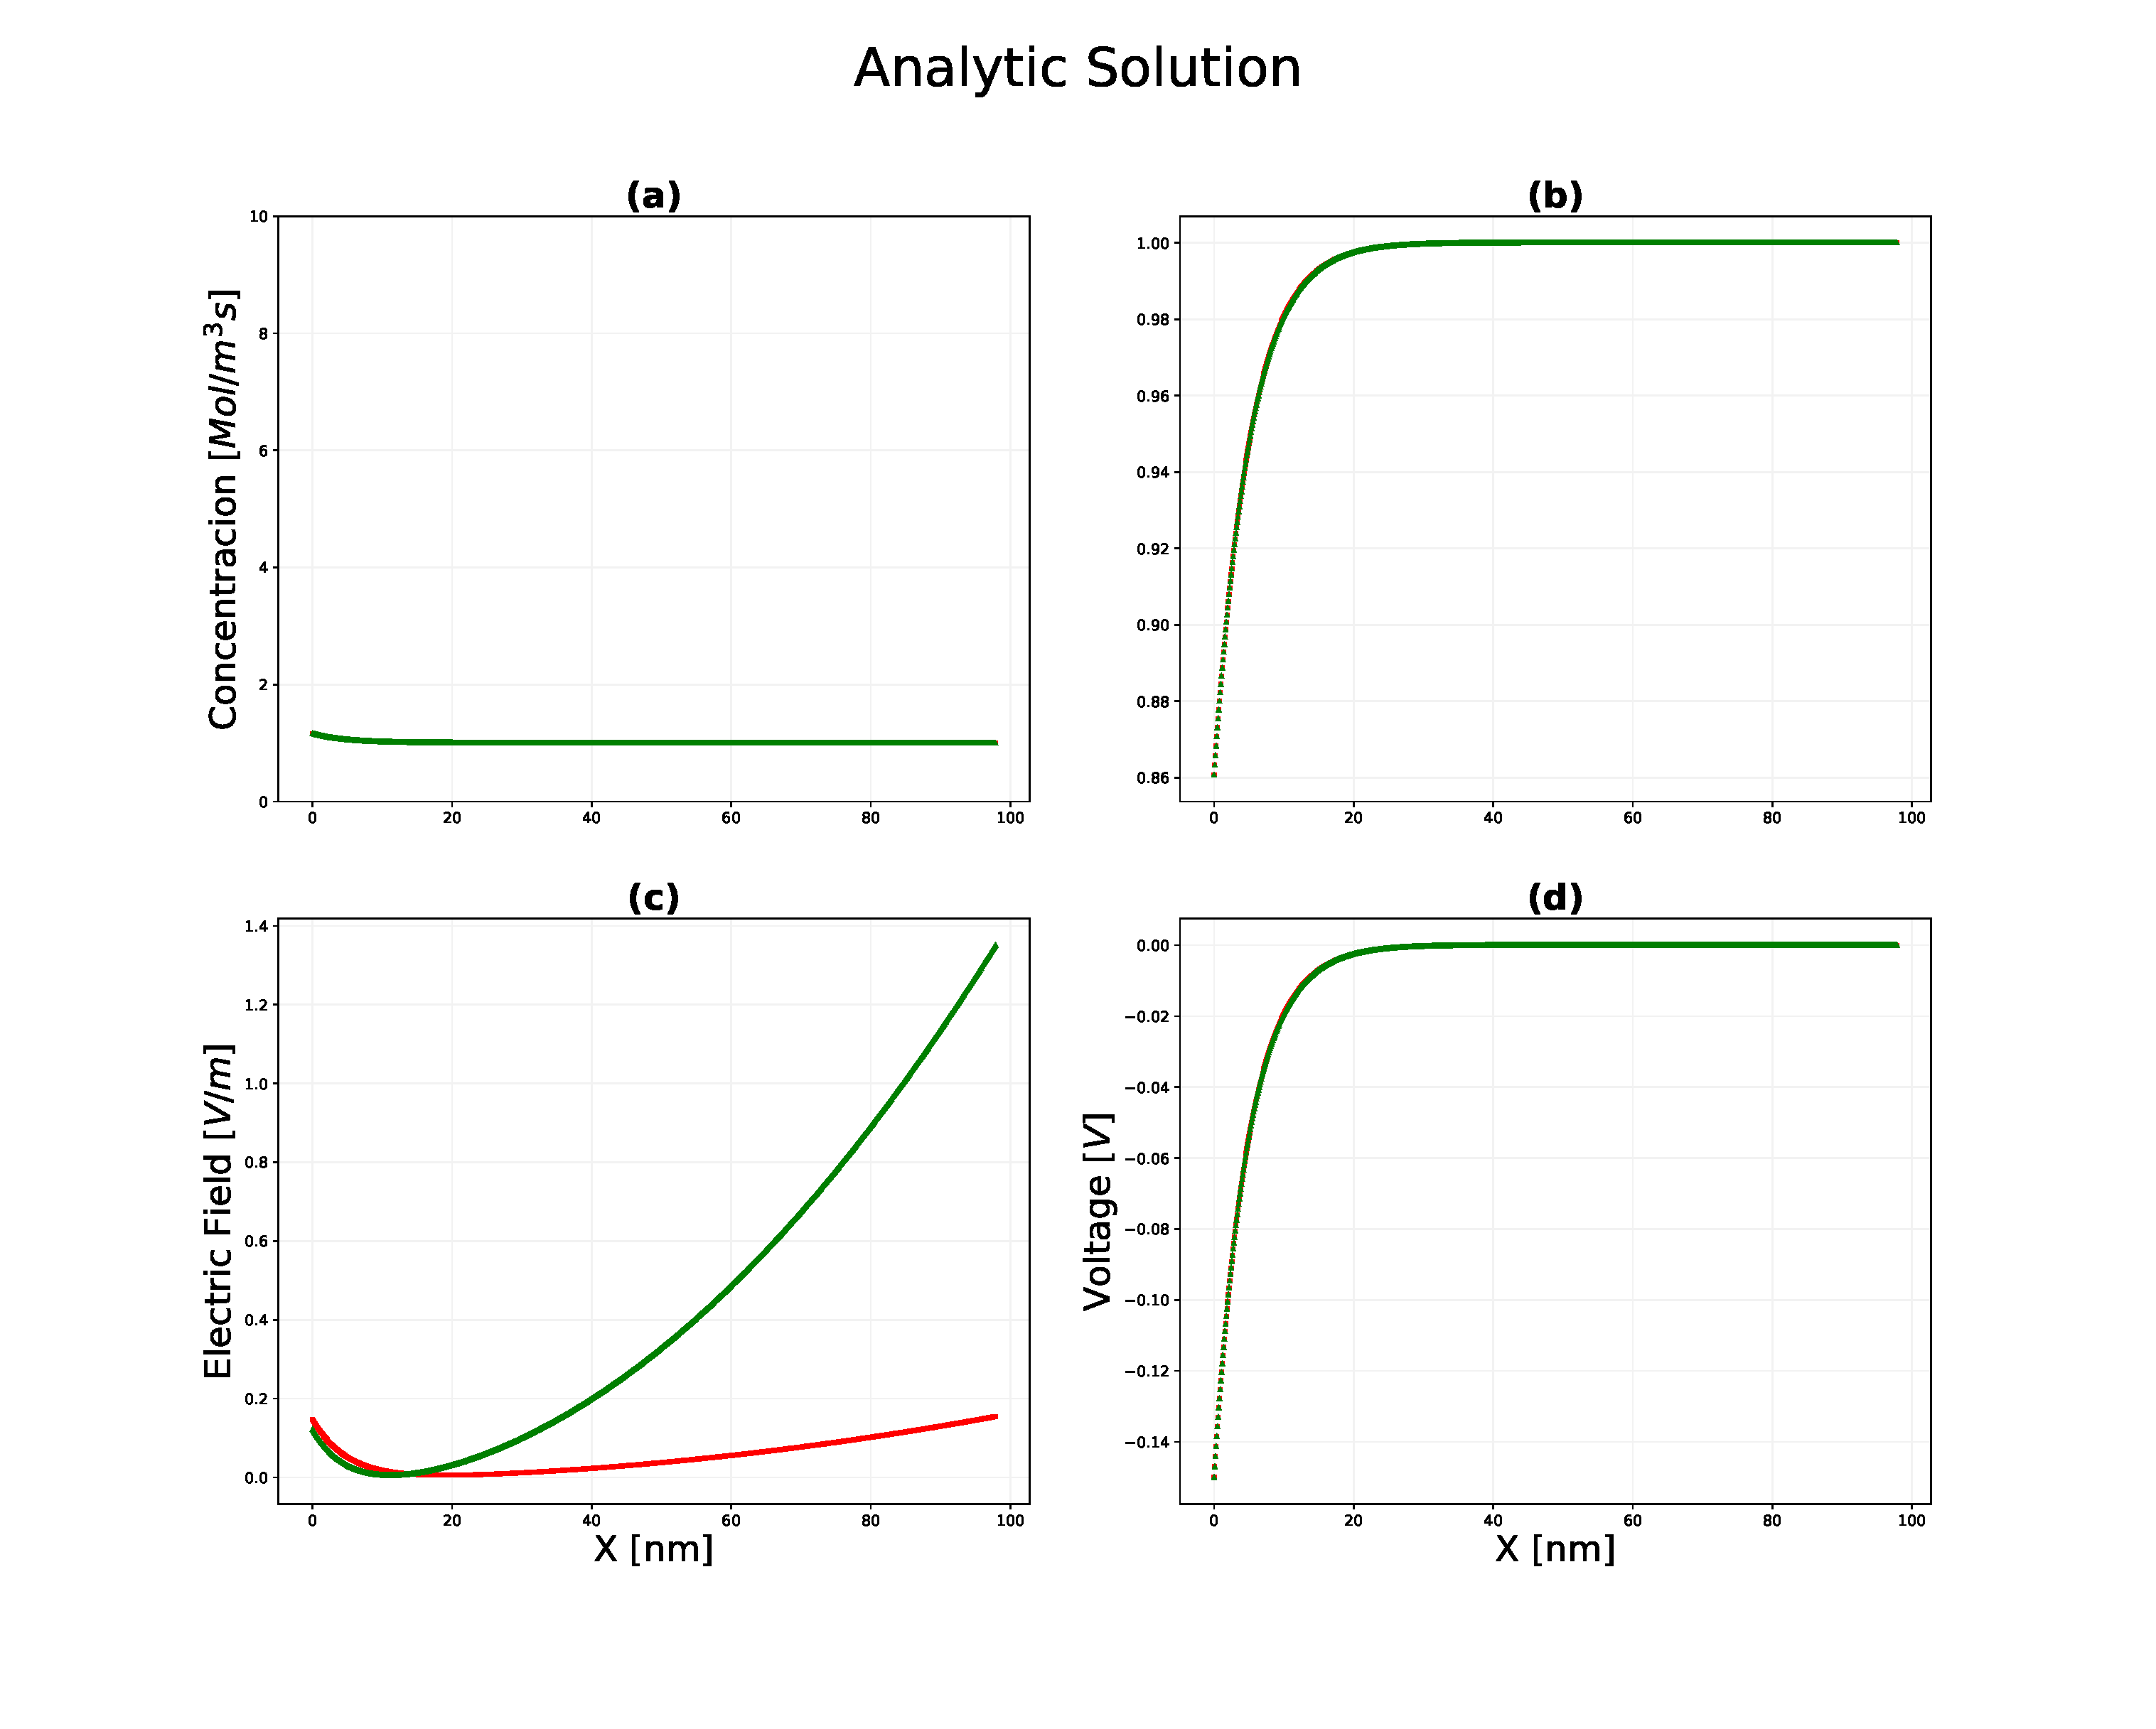
\includegraphics[width = \linewidth]{analytic-results}
 \caption{Analytic results. (a), (b) are the concentrations of each species of electrolytes. (c) is the electric potential and (d) the electric potential. Each plot is compared for 3 different values of the reaction rate.}
 \label{fig:analytic-results}
\end{figure}



